\documentclass{article}
\usepackage[utf8]{inputenc}
\usepackage{geometry}
\usepackage{amsmath, amsfonts, amssymb}
\usepackage{graphicx}
\usepackage{listings}
\usepackage{hyperref}
\usepackage{booktabs}
\usepackage{caption}
\usepackage{subcaption}
\usepackage{float}
\usepackage{natbib}
\usepackage{color}
\usepackage{courier}

\geometry{margin=1in}
\lstset{
    basicstyle=\footnotesize\ttfamily,
    breaklines=true,
    frame=single,
    numbers=left,
    numberstyle=\tiny,
    keywordstyle=\color{blue},
    commentstyle=\color{green!50!black},
    stringstyle=\color{red},
}

\title{Comprehensive Car Dataset Analysis}
\author{Your Name}
\date{\today}

\begin{document}

\maketitle

\tableofcontents

\section{Introduction}

In this report, we perform an end-to-end machine learning project using the car dataset. The analysis includes data exploration, preprocessing, feature engineering, modeling, evaluation, and visualization. We aim to predict the miles per gallon (MPG) for cars using regression models and classify whether a car is from Ford using classification models.

\section{Dataset Description}

The \textbf{Auto MPG Dataset} consists of 398 cars, including various technical specifications such as:

\begin{itemize}
    \item \textbf{mpg}: Miles per gallon (continuous)
    \item \textbf{cylinders}: Number of cylinders (multi-valued discrete)
    \item \textbf{displacement}: Engine displacement in cubic inches (continuous)
    \item \textbf{horsepower}: Engine horsepower (continuous)
    \item \textbf{weight}: Vehicle weight in pounds (continuous)
    \item \textbf{acceleration}: Time to accelerate from 0 to 60 mph (continuous)
    \item \textbf{model year}: Model year (multi-valued discrete)
    \item \textbf{origin}: Origin of the car (1: USA, 2: Europe, 3: Japan)
    \item \textbf{car name}: Car model name (string)
\end{itemize}

\textbf{Source}: The dataset is available from the UCI Machine Learning Repository.

\url{https://archive.ics.uci.edu/ml/datasets/auto+mpg}

\section{Data Loading and Exploration}

\subsection{Importing Libraries}

We start by importing the necessary libraries and ensuring compatibility.

\begin{lstlisting}[language=Python]
# Import necessary libraries
import sys
assert sys.version_info >= (3, 7)

from packaging import version
import sklearn
assert version.parse(sklearn.__version__) >= version.parse("1.0.1")

import pandas as pd
import numpy as np
import seaborn as sns
import matplotlib.pyplot as plt
import warnings

sns.set(style="whitegrid")
%matplotlib inline

warnings.filterwarnings('ignore')
np.random.seed(42)
\end{lstlisting}

\subsection{Loading the Dataset}

We load the dataset using Pandas.

\begin{lstlisting}[language=Python]
# Loading the car dataset
cars = pd.read_csv("cars.csv")

# Display the first few rows
cars.head()
\end{lstlisting}

\subsection{Data Overview}

We check data types and identify missing values.

\begin{lstlisting}[language=Python]
# Checking data types and missing values
cars.info()

# Summary statistics
cars.describe()
\end{lstlisting}

\section{Data Cleaning and Preprocessing}

\subsection{Handling Missing Values and Data Types}

We handle missing values in the \texttt{horsepower} column and convert data types.

\begin{lstlisting}[language=Python]
# Replace '?' with NaN and convert 'horsepower' to numeric
cars['horsepower'].replace('?', np.nan, inplace=True)
cars['horsepower'] = pd.to_numeric(cars['horsepower'], errors='coerce')

# Impute missing 'horsepower' with median
median_horsepower = cars['horsepower'].median()
cars['horsepower'].fillna(median_horsepower, inplace=True)

# Convert 'origin' to categorical
cars['origin'] = cars['origin'].map({1: 'USA', 2: 'Europe', 3: 'Japan'})

# Extract 'manufacturer' from 'car name'
cars['manufacturer'] = cars['car name'].str.split().str[0]

# Display cleaned dataset
cars.head()
\end{lstlisting}

\subsection{Handling Outliers}

We detect and remove outliers using the z-score method.

\begin{lstlisting}[language=Python]
# Detecting outliers using z-score
from scipy import stats

z_scores = stats.zscore(cars.select_dtypes(include=[np.number]))
abs_z_scores = np.abs(z_scores)
filtered_entries = (abs_z_scores < 3).all(axis=1)
cars = cars[filtered_entries]

print("Dataset shape after removing outliers:", cars.shape)
\end{lstlisting}

\section{Exploratory Data Analysis (EDA)}

\subsection{Distribution of MPG}

We visualize the distribution of the target variable \texttt{mpg}.

\begin{lstlisting}[language=Python]
# Distribution of MPG
plt.figure(figsize=(10, 6))
sns.histplot(cars["mpg"], bins=30, kde=True, color='blue', alpha=0.7)
plt.xlabel("Miles Per Gallon (MPG)")
plt.ylabel("Frequency")
plt.title("Distribution of MPG")
plt.savefig("mpg_distribution.png")
plt.show()
\end{lstlisting}

\begin{figure}[H]
    \centering
    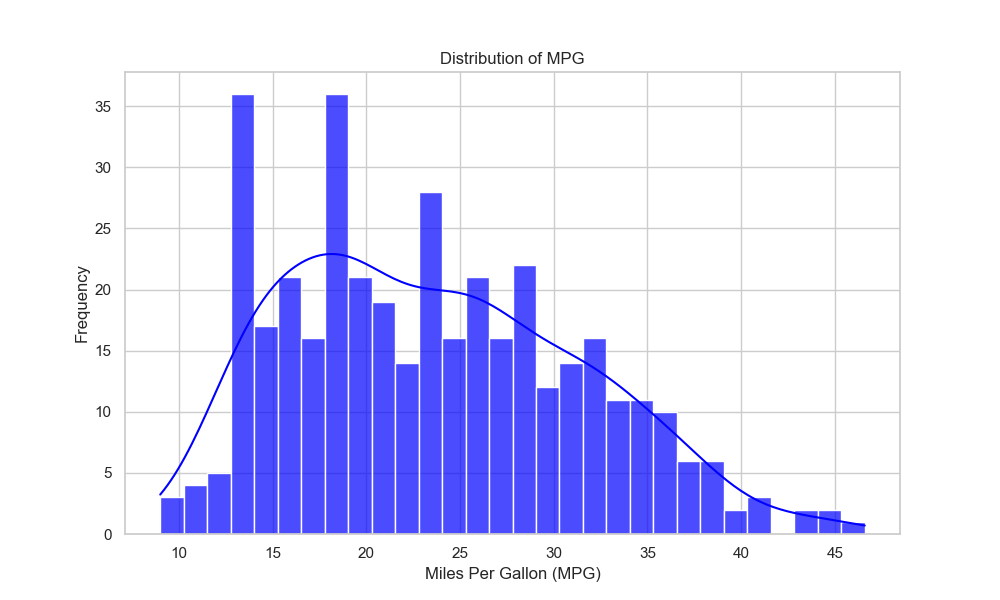
\includegraphics[width=0.7\textwidth]{mpg_distribution.png}
    \caption{Distribution of MPG}
\end{figure}

\subsection{Correlation Matrix}

We compute and visualize the correlation matrix.

\begin{lstlisting}[language=Python]
# Correlation Matrix
plt.figure(figsize=(12, 10))
corr_matrix = cars.corr()
sns.heatmap(corr_matrix, annot=True, cmap='coolwarm')
plt.title('Correlation Matrix')
plt.savefig('correlation_matrix.png')
plt.show()
\end{lstlisting}

\begin{figure}[H]
    \centering
    \includegraphics[width=0.9\textwidth]{correlation_matrix.png}
    \caption{Correlation Matrix}
\end{figure}

\subsection{Pair Plot}

We create pair plots to visualize relationships between features.

\begin{lstlisting}[language=Python]
# Pair Plot
sns.pairplot(cars[['mpg', 'horsepower', 'weight', 'acceleration', 'displacement']])
plt.savefig('pair_plot.png')
plt.show()
\end{lstlisting}

\begin{figure}[H]
    \centering
    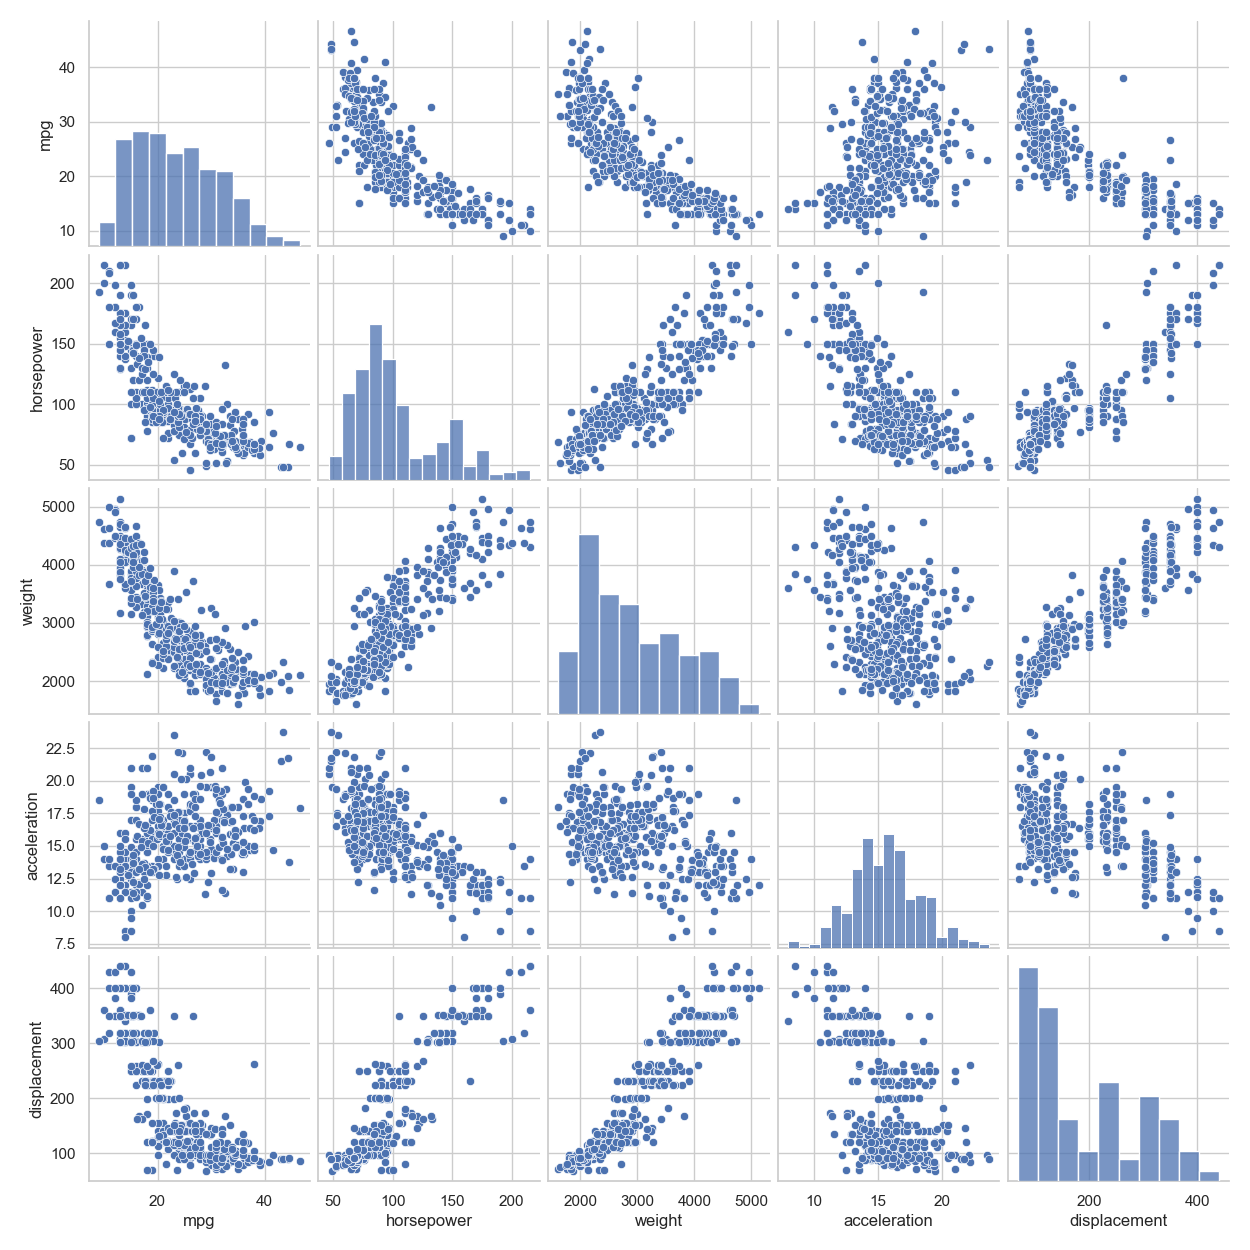
\includegraphics[width=0.9\textwidth]{pair_plot.png}
    \caption{Pair Plot of Selected Features}
\end{figure}

\subsection{Manufacturer Distribution}

We analyze the distribution of car manufacturers.

\begin{lstlisting}[language=Python]
# Distribution of Car Manufacturers
plt.figure(figsize=(12, 8))
top_manufacturers = cars['manufacturer'].value_counts().nlargest(20)
sns.barplot(x=top_manufacturers.index, y=top_manufacturers.values, palette="viridis")
plt.xticks(rotation=45)
plt.xlabel("Car Manufacturer")
plt.ylabel("Number of Cars")
plt.title("Top 20 Car Manufacturers in the Dataset")
plt.tight_layout()
plt.savefig("manufacturer_distribution.png")
plt.show()
\end{lstlisting}

\begin{figure}[H]
    \centering
    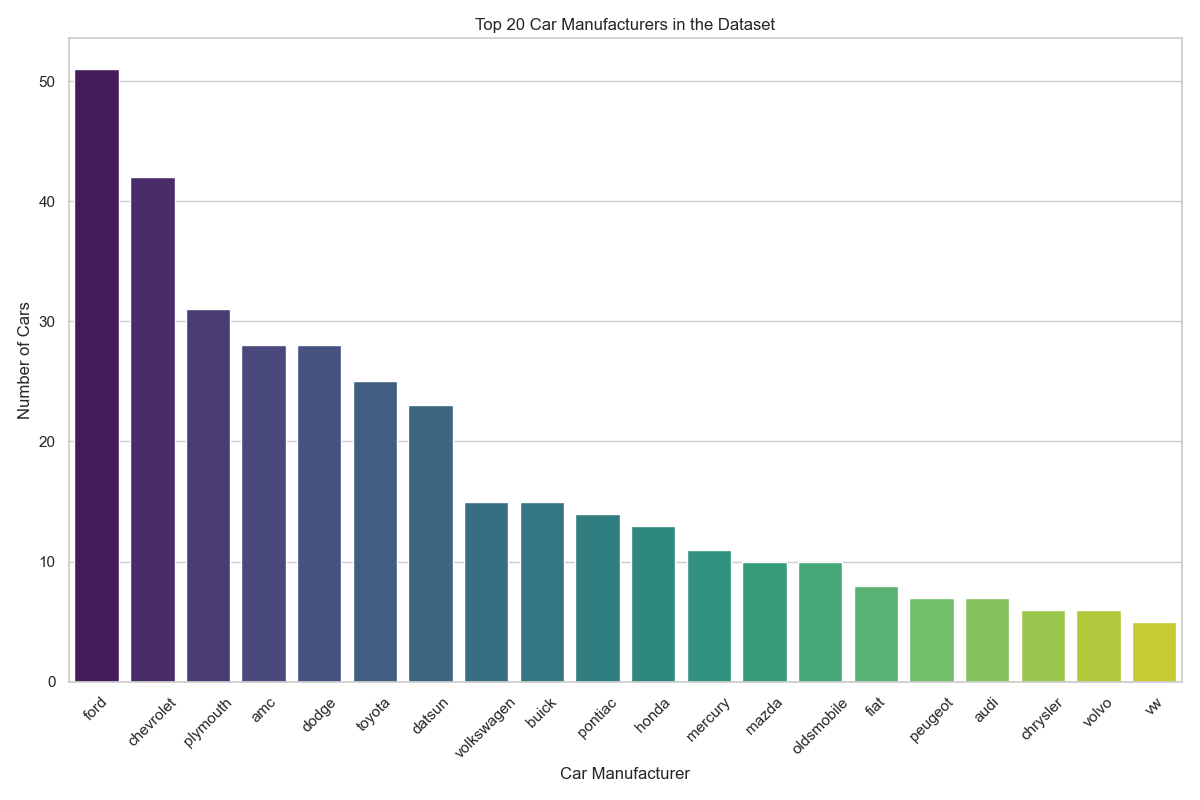
\includegraphics[width=0.9\textwidth]{manufacturer_distribution.png}
    \caption{Top 20 Car Manufacturers}
\end{figure}

\subsection{Class Imbalance Analysis}

We examine the class distribution for the classification task.

\begin{lstlisting}[language=Python]
# Class Imbalance Analysis
cars['is_ford'] = (cars['manufacturer'] == 'ford').astype(int)
class_counts = cars['is_ford'].value_counts()
print("Class Distribution:")
print(class_counts)

plt.figure(figsize=(6, 4))
sns.barplot(x=class_counts.index, y=class_counts.values)
plt.xticks([0, 1], ['Not Ford', 'Ford'])
plt.xlabel('Car Type')
plt.ylabel('Count')
plt.title('Ford vs. Not Ford Distribution')
plt.savefig('class_distribution.png')
plt.show()
\end{lstlisting}

\begin{figure}[H]
    \centering
    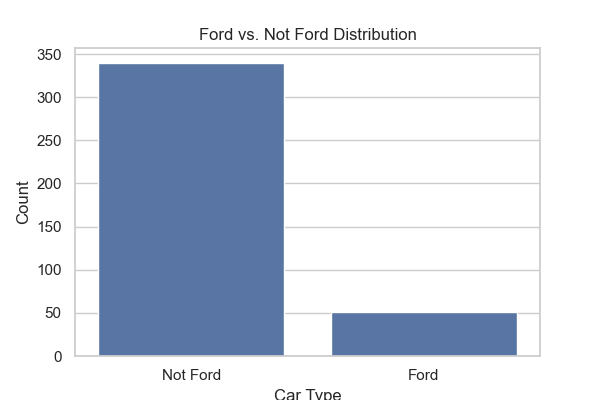
\includegraphics[width=0.6\textwidth]{class_distribution.png}
    \caption{Ford vs. Not Ford Distribution}
\end{figure}

\section{Feature Engineering}

\subsection{Creating New Features}

We engineer new features to enhance model performance.

\begin{itemize}
    \item \textbf{Power-to-Weight Ratio}:
    \[
    \text{Power-to-Weight Ratio} = \frac{\text{Horsepower}}{\text{Weight}}
    \]
    \item \textbf{Displacement per Cylinder}:
    \[
    \text{Displacement per Cylinder} = \frac{\text{Displacement}}{\text{Cylinders}}
    \]
\end{itemize}

\begin{lstlisting}[language=Python]
# Creating power-to-weight ratio
cars['power_to_weight'] = cars['horsepower'] / cars['weight']

# Creating displacement per cylinder
cars['displacement_per_cylinder'] = cars['displacement'] / cars['cylinders']

# Encoding categorical variables
cars = pd.get_dummies(cars, columns=['origin'], drop_first=True)

cars.head()
\end{lstlisting}

\section{Defining Features and Splitting Data}

\subsection{Preparing Features and Targets}

We define the feature set and target variables for regression and classification.

\begin{lstlisting}[language=Python]
# Defining features and target for regression
features = ['horsepower', 'weight', 'acceleration', 'displacement', 
            'power_to_weight', 'displacement_per_cylinder', 
            'origin_Europe', 'origin_Japan']
X_regression = cars[features]
y_regression = cars['mpg']

# Defining features and target for classification
X_classification = cars[features]
y_classification = cars['is_ford']
\end{lstlisting}

\subsection{Splitting the Data}

We split the data into training and testing sets.

\begin{lstlisting}[language=Python]
# Splitting the data into training and testing sets
from sklearn.model_selection import train_test_split

# Regression data split
X_train_reg, X_test_reg, y_train_reg, y_test_reg = train_test_split(
    X_regression, y_regression, test_size=0.2, random_state=42
)

# Classification data split
X_train_clf, X_test_clf, y_train_clf, y_test_clf = train_test_split(
    X_classification, y_classification, test_size=0.2, random_state=42, stratify=y_classification
)
\end{lstlisting}

\section{Modeling and Evaluation}

\subsection{Regression Models}

\subsubsection{Linear Regression}

We train a Linear Regression model and evaluate its performance.

\begin{lstlisting}[language=Python]
# Linear Regression Model
from sklearn.linear_model import LinearRegression
from sklearn.metrics import mean_squared_error, mean_absolute_error, r2_score

lin_reg = LinearRegression()
lin_reg.fit(X_train_reg, y_train_reg)

# Predictions and Evaluation
y_pred_lin_reg = lin_reg.predict(X_test_reg)
mse_lin_reg = mean_squared_error(y_test_reg, y_pred_lin_reg)
mae_lin_reg = mean_absolute_error(y_test_reg, y_pred_lin_reg)
r2_lin_reg = r2_score(y_test_reg, y_pred_lin_reg)

print("Linear Regression Evaluation:")
print(f"MSE: {mse_lin_reg:.2f}")
print(f"MAE: {mae_lin_reg:.2f}")
print(f"R^2 Score: {r2_lin_reg:.2f}")
\end{lstlisting}

\textbf{Linear Regression Equations}:

The prediction is made using:

\[
\hat{y} = X \beta + \epsilon
\]

where:
\begin{itemize}
    \item \( X \) is the feature matrix
    \item \( \beta \) are the coefficients
    \item \( \epsilon \) is the error term
\end{itemize}

\subsubsection{Random Forest Regression}

We train a Random Forest Regression model.

\begin{lstlisting}[language=Python]
# Random Forest Regression
from sklearn.ensemble import RandomForestRegressor

rf_reg = RandomForestRegressor(random_state=42)
rf_reg.fit(X_train_reg, y_train_reg)

# Predictions and Evaluation
y_pred_rf_reg = rf_reg.predict(X_test_reg)
mse_rf_reg = mean_squared_error(y_test_reg, y_pred_rf_reg)
mae_rf_reg = mean_absolute_error(y_test_reg, y_pred_rf_reg)
r2_rf_reg = r2_score(y_test_reg, y_pred_rf_reg)

print("Random Forest Regression Evaluation:")
print(f"MSE: {mse_rf_reg:.2f}")
print(f"MAE: {mae_rf_reg:.2f}")
print(f"R^2 Score: {r2_rf_reg:.2f}")
\end{lstlisting}

\textbf{Random Forest Regression} combines multiple decision trees to improve predictive accuracy and control over-fitting.

\subsubsection{Support Vector Regression}

We train a Support Vector Regression (SVR) model.

\begin{lstlisting}[language=Python]
# Support Vector Regression
from sklearn.svm import SVR

svr_reg = SVR()
svr_reg.fit(X_train_reg, y_train_reg)

# Predictions and Evaluation
y_pred_svr_reg = svr_reg.predict(X_test_reg)
mse_svr_reg = mean_squared_error(y_test_reg, y_pred_svr_reg)
mae_svr_reg = mean_absolute_error(y_test_reg, y_pred_svr_reg)
r2_svr_reg = r2_score(y_test_reg, y_pred_svr_reg)

print("Support Vector Regression Evaluation:")
print(f"MSE: {mse_svr_reg:.2f}")
print(f"MAE: {mae_svr_reg:.2f}")
print(f"R^2 Score: {r2_svr_reg:.2f}")
\end{lstlisting}

\subsection{Classification Models}

\subsubsection{Logistic Regression}

We train a Logistic Regression model.

\begin{lstlisting}[language=Python]
# Logistic Regression Model
from sklearn.linear_model import LogisticRegression
from sklearn.metrics import accuracy_score, precision_score, recall_score, f1_score, classification_report

log_reg = LogisticRegression(max_iter=1000)
log_reg.fit(X_train_clf, y_train_clf)

# Predictions and Evaluation
y_pred_log_reg = log_reg.predict(X_test_clf)
accuracy_log_reg = accuracy_score(y_test_clf, y_pred_log_reg)
precision_log_reg = precision_score(y_test_clf, y_pred_log_reg)
recall_log_reg = recall_score(y_test_clf, y_pred_log_reg)
f1_log_reg = f1_score(y_test_clf, y_pred_log_reg)

print("Logistic Regression Evaluation:")
print(f"Accuracy: {accuracy_log_reg:.2f}")
print(f"Precision: {precision_log_reg:.2f}")
print(f"Recall: {recall_log_reg:.2f}")
print(f"F1 Score: {f1_log_reg:.2f}")
print("\nClassification Report:")
print(classification_report(y_test_clf, y_pred_log_reg))
\end{lstlisting}

\textbf{Logistic Regression Equation}:

The probability of the positive class is modeled as:

\[
p = \frac{1}{1 + e^{- (X \beta)}}
\]

\subsubsection{Random Forest Classification}

We train a Random Forest Classifier.

\begin{lstlisting}[language=Python]
# Random Forest Classification
from sklearn.ensemble import RandomForestClassifier

rf_clf = RandomForestClassifier(random_state=42)
rf_clf.fit(X_train_clf, y_train_clf)

# Predictions and Evaluation
y_pred_rf_clf = rf_clf.predict(X_test_clf)
accuracy_rf_clf = accuracy_score(y_test_clf, y_pred_rf_clf)
precision_rf_clf = precision_score(y_test_clf, y_pred_rf_clf)
recall_rf_clf = recall_score(y_test_clf, y_pred_rf_clf)
f1_rf_clf = f1_score(y_test_clf, y_pred_rf_clf)

print("Random Forest Classification Evaluation:")
print(f"Accuracy: {accuracy_rf_clf:.2f}")
print(f"Precision: {precision_rf_clf:.2f}")
print(f"Recall: {recall_rf_clf:.2f}")
print(f"F1 Score: {f1_rf_clf:.2f}")
print("\nClassification Report:")
print(classification_report(y_test_clf, y_pred_rf_clf))
\end{lstlisting}

\subsubsection{Support Vector Classification}

We train a Support Vector Classifier.

\begin{lstlisting}[language=Python]
# Support Vector Classification
from sklearn.svm import SVC

svc_clf = SVC(probability=True)
svc_clf.fit(X_train_clf, y_train_clf)

# Predictions and Evaluation
y_pred_svc_clf = svc_clf.predict(X_test_clf)
accuracy_svc_clf = accuracy_score(y_test_clf, y_pred_svc_clf)
precision_svc_clf = precision_score(y_test_clf, y_pred_svc_clf)
recall_svc_clf = recall_score(y_test_clf, y_pred_svc_clf)
f1_svc_clf = f1_score(y_test_clf, y_pred_svc_clf)

print("Support Vector Classification Evaluation:")
print(f"Accuracy: {accuracy_svc_clf:.2f}")
print(f"Precision: {precision_svc_clf:.2f}")
print(f"Recall: {recall_svc_clf:.2f}")
print(f"F1 Score: {f1_svc_clf:.2f}")
print("\nClassification Report:")
print(classification_report(y_test_clf, y_pred_svc_clf))
\end{lstlisting}

\section{Hyperparameter Tuning}

\subsection{Random Forest Regression Tuning}

We use GridSearchCV to fine-tune the Random Forest Regression model.

\begin{lstlisting}[language=Python]
# Hyperparameter Tuning for Random Forest Regression
from sklearn.model_selection import GridSearchCV

param_grid_rf_reg = {
    'n_estimators': [50, 100, 200],
    'max_depth': [None, 5, 10],
    'min_samples_split': [2, 5, 10]
}

grid_search_rf_reg = GridSearchCV(RandomForestRegressor(random_state=42), param_grid_rf_reg, cv=5)
grid_search_rf_reg.fit(X_train_reg, y_train_reg)

print("Best Parameters for Random Forest Regression:")
print(grid_search_rf_reg.best_params_)

# Evaluating the tuned model
y_pred_rf_reg_tuned = grid_search_rf_reg.predict(X_test_reg)
mse_rf_reg_tuned = mean_squared_error(y_test_reg, y_pred_rf_reg_tuned)
mae_rf_reg_tuned = mean_absolute_error(y_test_reg, y_pred_rf_reg_tuned)
r2_rf_reg_tuned = r2_score(y_test_reg, y_pred_rf_reg_tuned)

print("Tuned Random Forest Regression Evaluation:")
print(f"MSE: {mse_rf_reg_tuned:.2f}")
print(f"MAE: {mae_rf_reg_tuned:.2f}")
print(f"R^2 Score: {r2_rf_reg_tuned:.2f}")
\end{lstlisting}

\section{Results Visualization}

\subsection{Regression Results Plot}

We plot the actual vs. predicted MPG values for the tuned Random Forest Regression model.

\begin{lstlisting}[language=Python]
# Plotting Actual vs Predicted MPG for Random Forest Regression
plt.figure(figsize=(10, 6))
sns.scatterplot(x=y_test_reg, y=y_pred_rf_reg_tuned, alpha=0.7, color='red')
plt.plot([y_test_reg.min(), y_test_reg.max()], [y_test_reg.min(), y_test_reg.max()], 'k--',